\textbf{Rescaling torque-signal}\\
As the PSoC can only measure voltage-levels ranging from $0$ to $+5 V$, and the output-signal from the torque measurement lies between $-5 V$ to $+5 V$, it is necessary to rescale the signal such that the PSoC's input-signal can be described using this formula:
\begin{equation}
	V_t = \frac{\tau_{sensor} }{2} + 2.5 V
\end{equation}

The desired signal can be found by amplifying the input-signal with a factor 0.5 and then lifting the signal with an offset of $\SI{2.5}{\volt}$. This can be done using a non-inverting adder.

\begin{figure}[H]
	\centering
	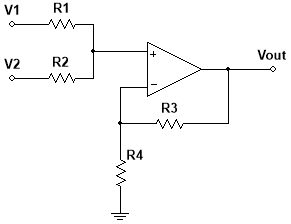
\includegraphics[width=0.4\linewidth]{Hardware/SignalConverter/TorqueDesign1}
	\caption{Non-inverting adder using operational amplifier}
	\label{fig:SignalConverterTorque1}
\end{figure}

A non-inverting adder is similiar to a non-inverting amplifier but contains a voltage divider on the Op-amps non-inverting input. The design is based on equally sized resistors:
\begin{equation}
	R_1 = R_2 = R_3 = R_4
\end{equation}
Due to the high-impedance of the op-amp, no current flows into the input. he current I\textsubscript{P} can be therefore bee calculated using Ohm's law:
\begin{equation}
	I_P = \frac{V_1 - V_2}{R_1 + R_2} = \frac{V_1 - V_2}{2 \cdot R}
\end{equation}
The voltage on the op-amps non-inverting input can be calculated as:
\begin{equation}
	V_P = V_1 - V_2 = V_1 - I_P \cdot R = V_1 - \frac{V_1 - V_2}{2 \cdot R} \cdot R = \frac{V_1 + V_2}{2}
\end{equation}
Due to the op-amps negative feedback it function as a non-inverting amplifier. This amplification can be found as:
\begin{equation}
	A = 1 + \frac{R}{R} = 2
\end{equation}
This means that the op-amps output-voltage can be calculated as:
\begin{equation}
	V_{out} = V_P \cdot A = \frac{V_1 + V_2}{2} \cdot 2 = V_1 + V_2
\end{equation}
The signals V\textsubscript{1} is the $\pm \SI{5}{\volt}$ signal from the Torque Sensor. The signal's voltage is cut in half using a voltage divider. The signal V\textsubscript{2} is the 5 VDC supply which can be used to add a $\SI{2.5}{\volt}$ offset to the input. This is also done using a voltage divider. Both voltage dividers can be made using only $\SI{10}{\kilo \ohm}$ resistors. This resistor-value is also used in the rest of the design. This leads to the final design seen below:

\begin{figure}[H]
	\centering
	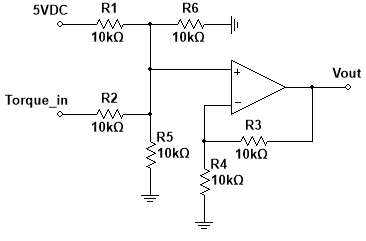
\includegraphics[width=0.5\linewidth]{Hardware/SignalConverter/TorqueDesign2}
	\caption{Circuit diagram for Signal Converter (torque-signal)}
	\label{fig:SignalConverterTorque2}
\end{figure}